\documentclass[10pt]{article}
\usepackage[top = 0.5in, bottom = 1.0in, left = 1.0in, right = 1.0in]{geometry}
\usepackage{float}
\usepackage{amsmath}
\usepackage{graphicx}
\usepackage{indentfirst}
\graphicspath{ {../figures/} }
\title{CS 418 Final Project}
\date{December 3, 2019}
\author {Manasa Kandimalla, Shyam Patel, Carlos Antonio McNulty}
\begin{document}
\maketitle

\section*{1. Problem Selection}

\section*{2. Data Collection}

\section*{3. Data Preparation}

\section*{4. Data Exploration}

\begin{figure}[H]
\caption{Drug Usage}
\centering
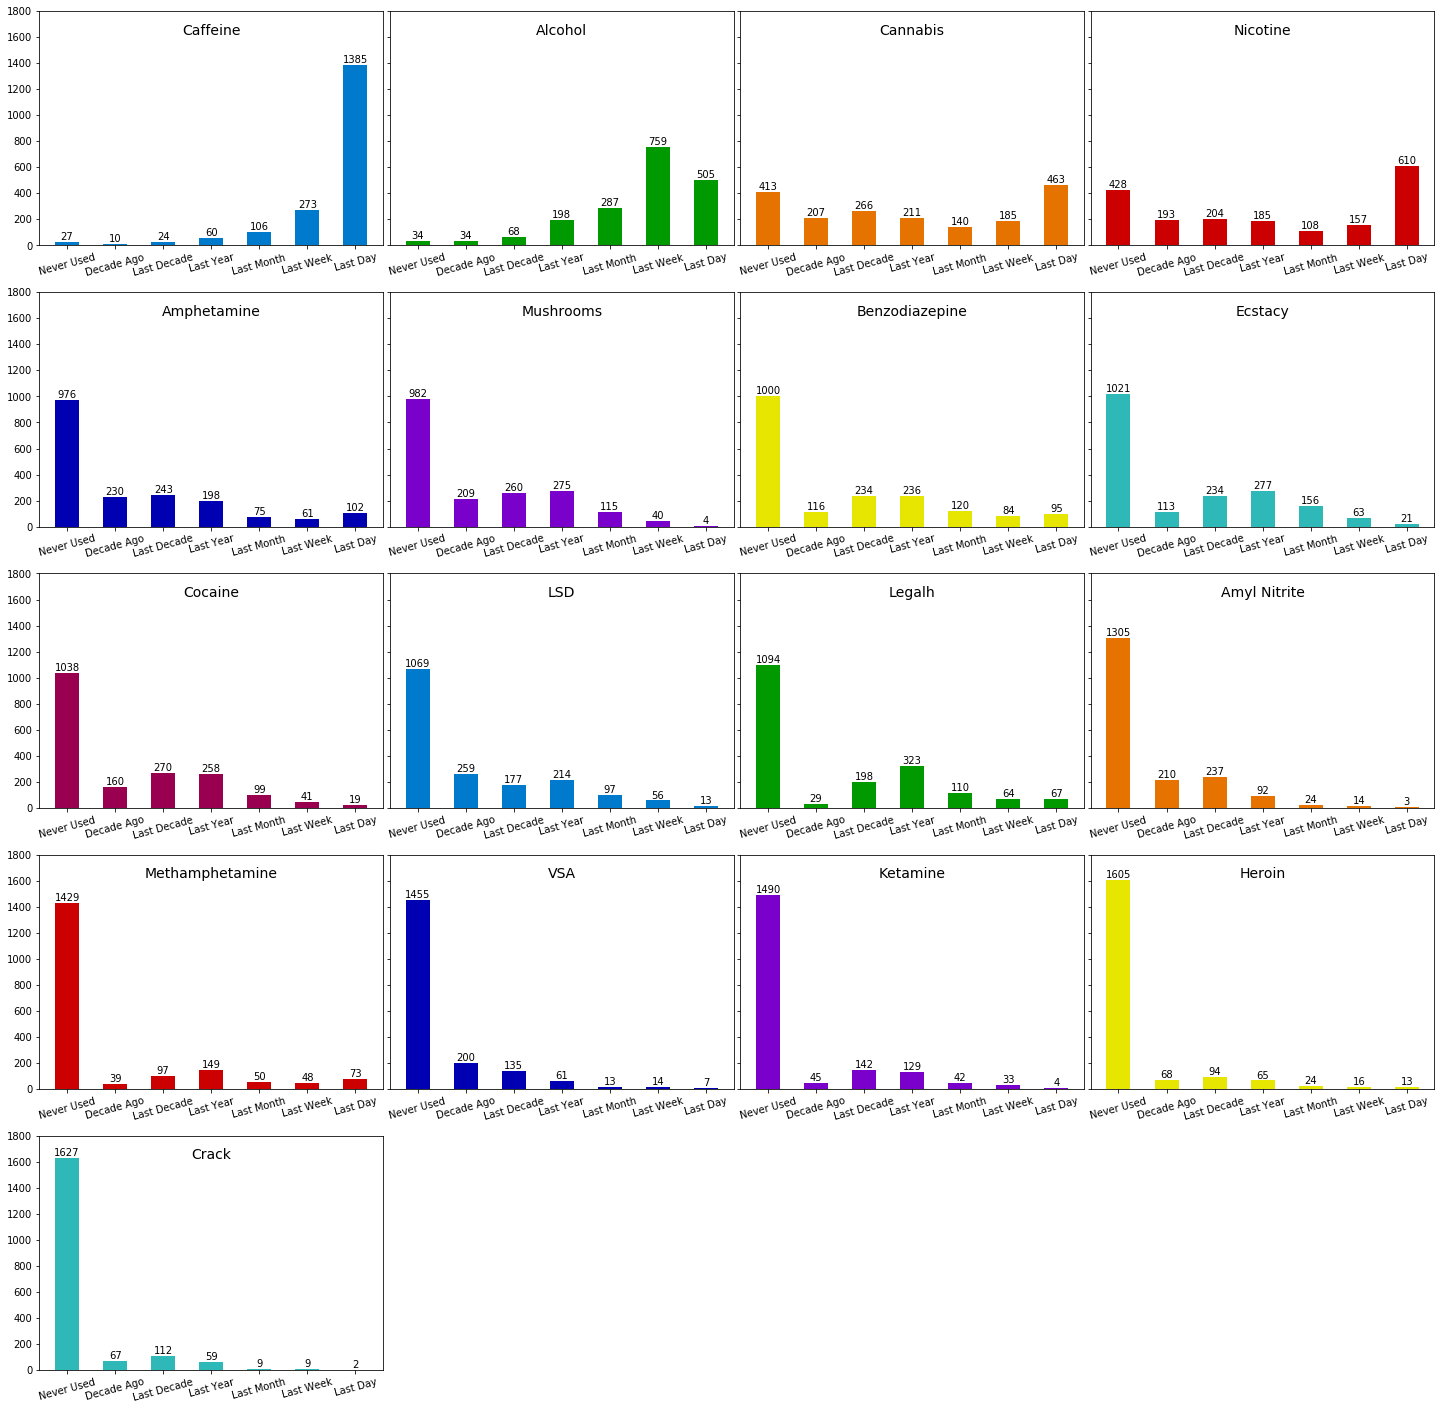
\includegraphics[scale=0.7]{drugs.png}
\end{figure}

\begin{figure}[H]
\caption{Illegal Drug Usage and Frequency by Gender}
\centering
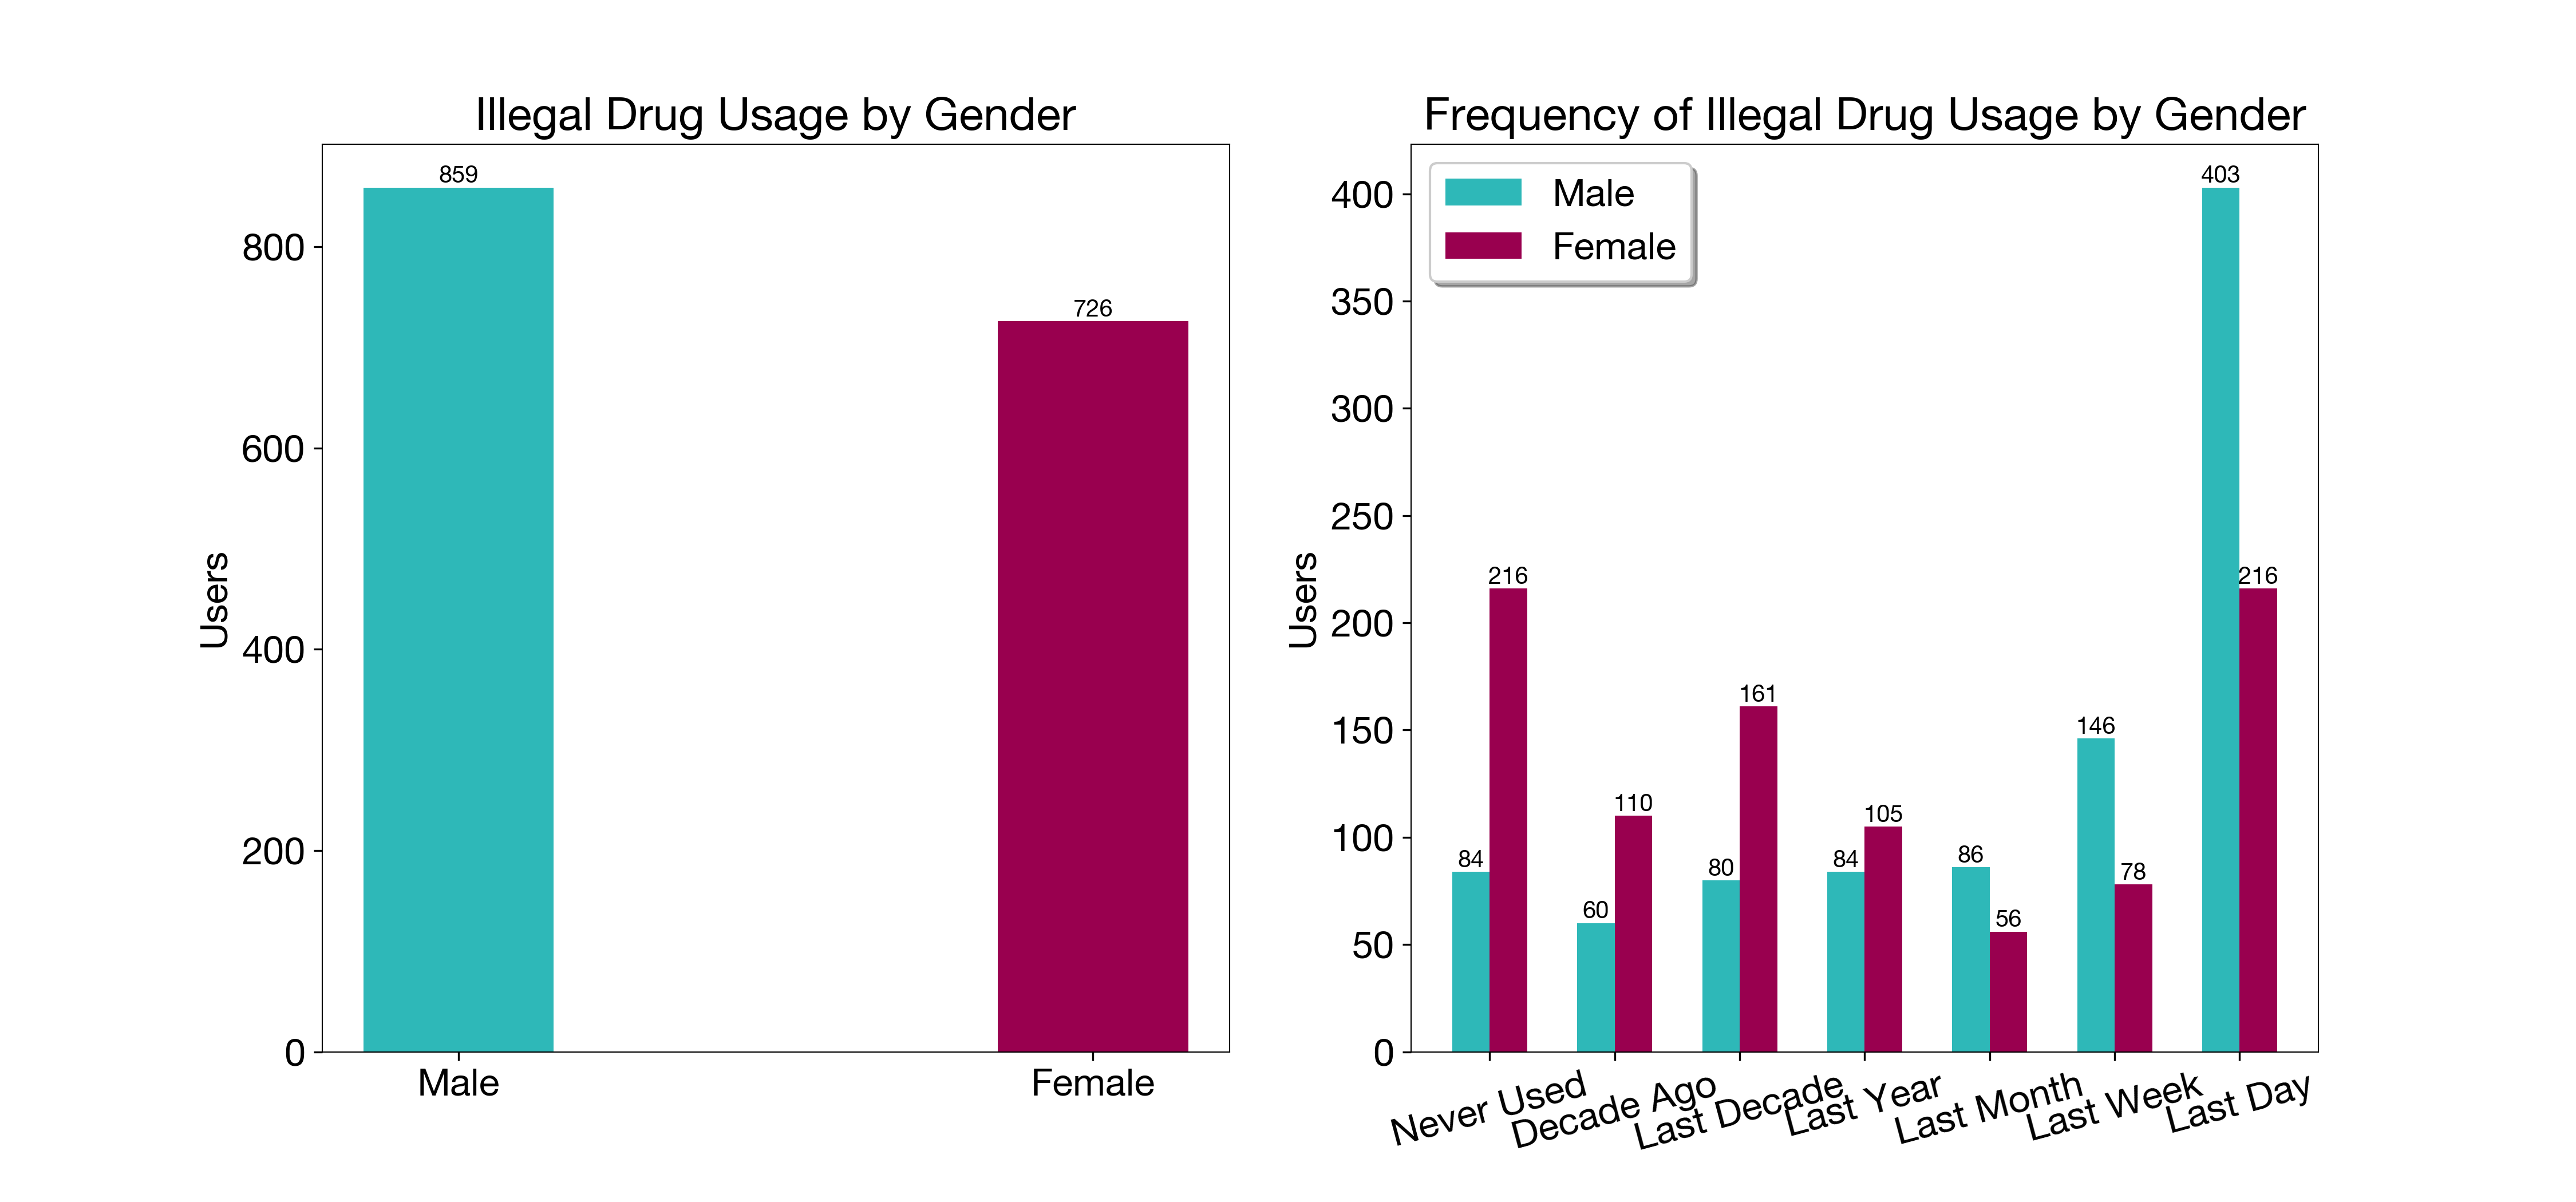
\includegraphics[scale=0.4]{gender_freq.png}
\end{figure}

\begin{figure}[H]
\caption{Illegal Drug Usage by Personality Trait}
\centering
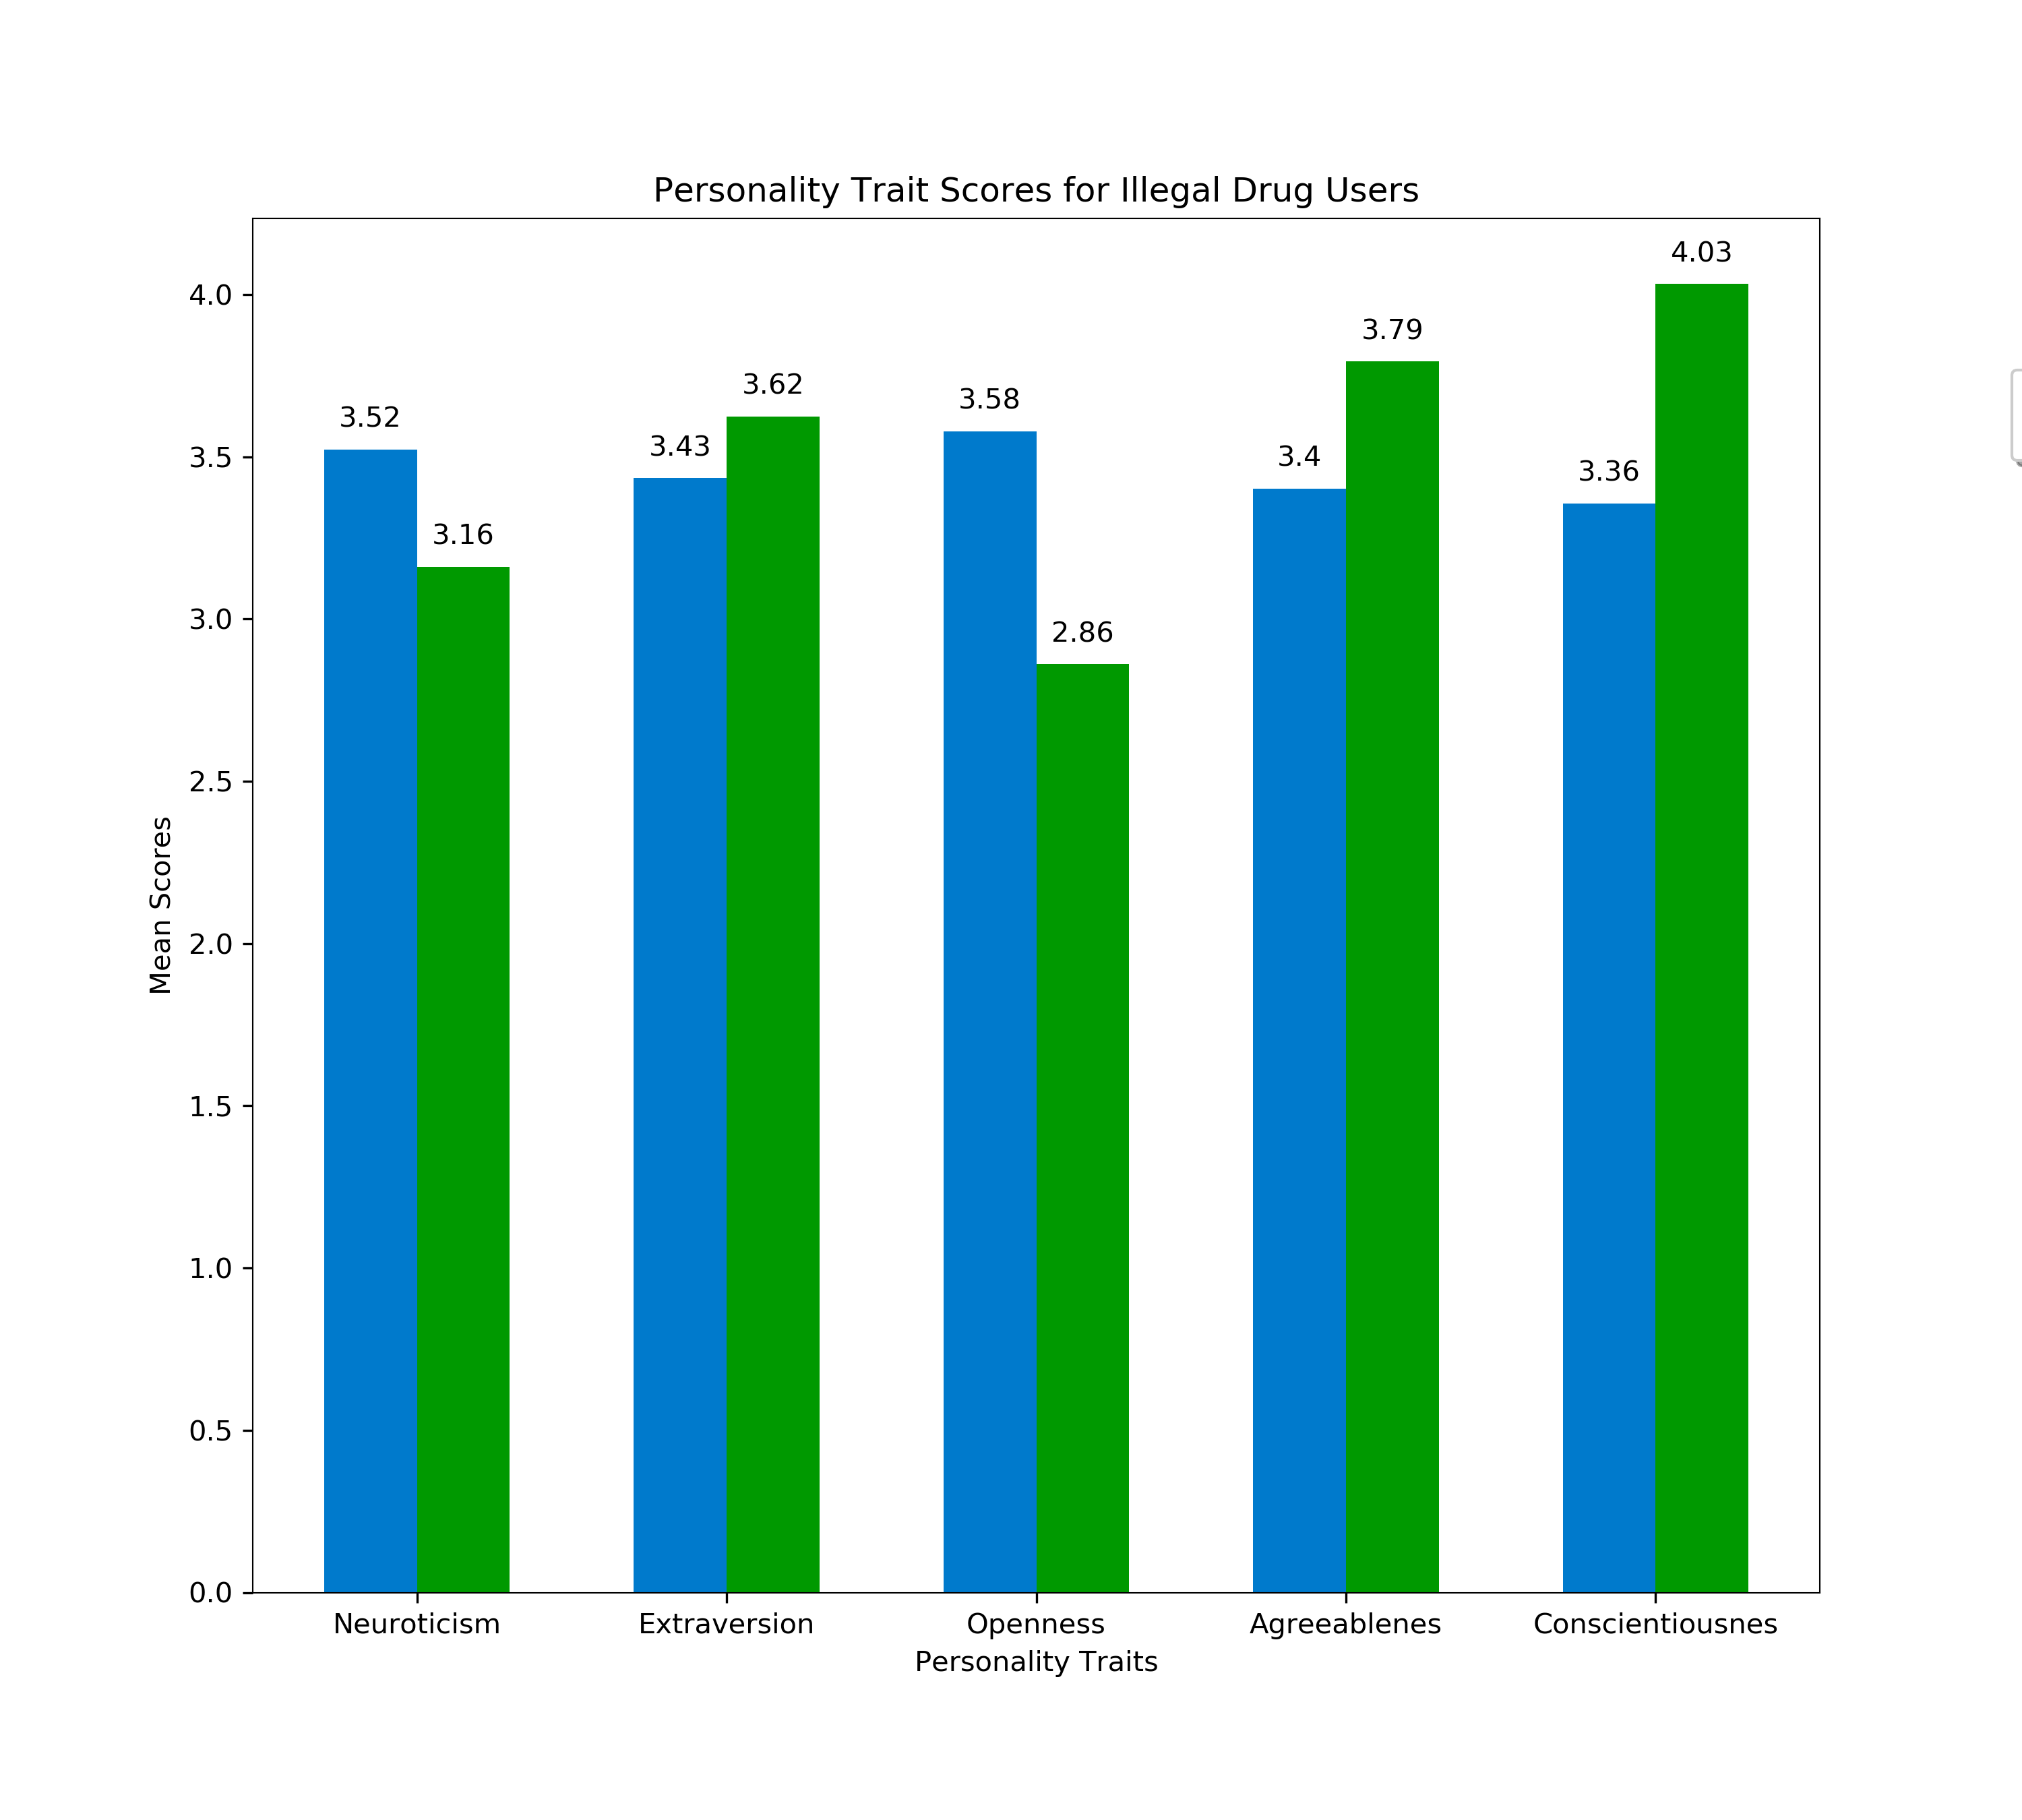
\includegraphics[scale=0.25]{traits.png}
\end{figure}

\begin{figure}[H]
\caption{Heatmap of Correlation Matrix}
\centering
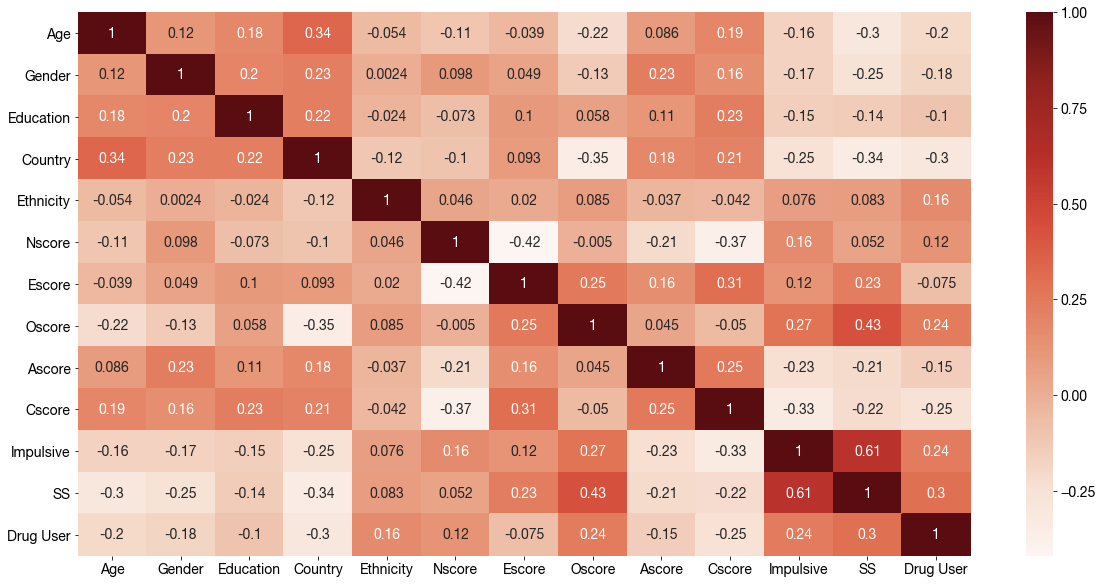
\includegraphics[scale=0.25]{heatmap.png}
\end{figure}

\section*{5. Data Modeling}

\subsection*{Decision Tree Classifier}

\subsection*{Random Forest Classifier}

\subsubsection*{Feature Selection}

\subsubsection*{Grid Search}

\begin{figure}[H]
\caption{Hyperparameter Tuning with Grid Search }
\centering
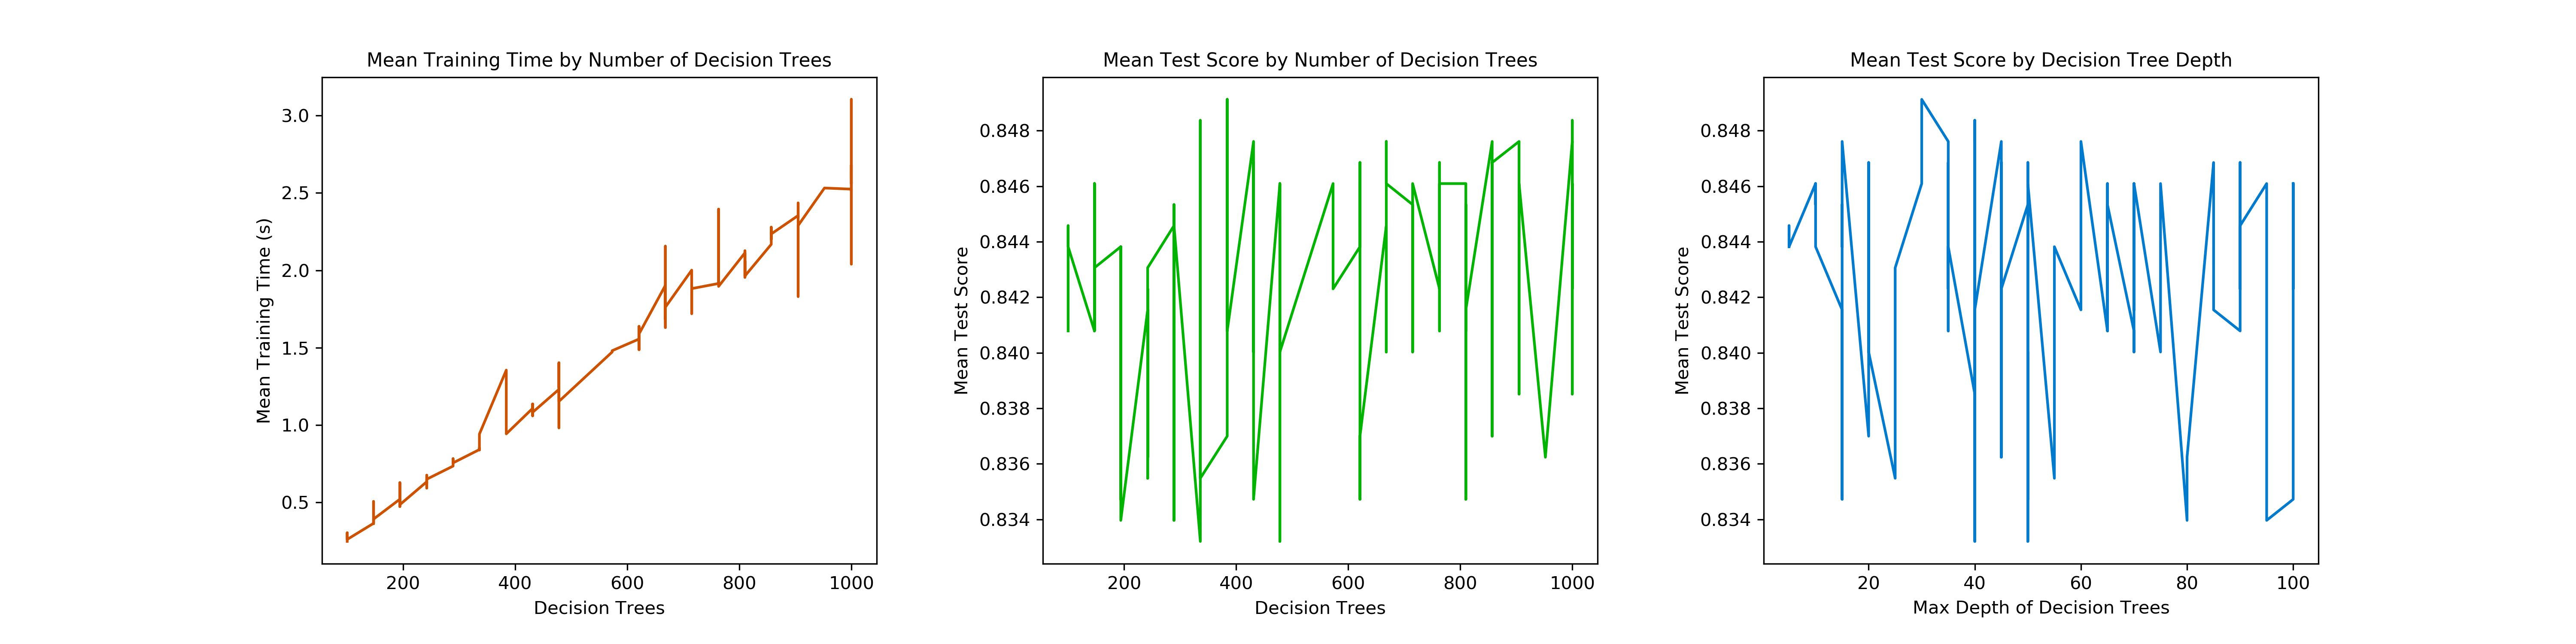
\includegraphics[scale=0.35]{gridsearch.png}
\end{figure}

We performed grid search on 30,240 random forests by varying the number of estimators and the configuration for the base estimators provided to each random forest.\par

\subsection*{Clustering}

\section*{6. Results}


\end{document}